\documentclass[aspectratio=169]{beamer}
\usepackage[utf8]{inputenc}
\usepackage[turkish]{babel}
\usepackage{amsmath}
\usepackage{amsfonts}
\usepackage{amssymb}
\usepackage{graphicx}
\usepackage{listings}
\usepackage{xcolor}
\usepackage{tikz}
\usetikzlibrary{positioning, shapes.geometric, arrows}
\usepackage{algorithm}
\usepackage{algorithmic}
\usepackage{hyperref}

% Beamer theme
\usetheme{Madrid}
\usecolortheme{default}

% Code styling
\lstset{
    backgroundcolor=\color{gray!10},
    basicstyle=\footnotesize\ttfamily,
    keywordstyle=\color{blue},
    commentstyle=\color{green!60!black},
    stringstyle=\color{red},
    showstringspaces=false,
    breaklines=true,
    frame=single,
    language=Python
}

% Title page
\title{LangGraph ile Sosyal Ağ Analizi: \\ Çizge Teorisi ve AI Ajanları}
\subtitle{Bilgisayar Mühendisliği Yüksek Lisans - Çizge Teorisi}
\author{[Öğrenci Adı]}
\institute{[Üniversite Adı]}
\date{\today}

\begin{document}

\frame{\titlepage}

% Table of Contents
\begin{frame}
\frametitle{İçindekiler}
\tableofcontents
\end{frame}

\section{Giriş ve Motivasyon}

\begin{frame}
\frametitle{Proje Motivasyonu}
\begin{itemize}
    \item \textbf{Problem:} Sosyal ağ verilerinin karmaşıklığı
    \item \textbf{Geleneksel Yaklaşım:} Manuel analiz ve yorumlama
    \item \textbf{Modern Çözüm:} AI destekli otomatik analiz
    \item \textbf{Hedef:} Çizge teorisi + Modern AI teknolojilerinin birleşimi
\end{itemize}

\vspace{0.5cm}
\begin{block}{Projenin Amacı}
LangGraph framework'ü kullanarak sosyal ağ analizini otomatikleştiren, doğal dil ile etkileşim kurabilen bir AI ajanı geliştirmek.
\end{block}
\end{frame}

\begin{frame}
\frametitle{Proje Avantajları}
\begin{columns}
\begin{column}{0.5\textwidth}
\textbf{Teorik Katkılar:}
\begin{itemize}
    \item Çizge teorisi kavramlarının uygulamalı kullanımı
    \item Merkezi önemi (centrality) ölçümlerinin karşılaştırılması
    \item Topluluk tespiti algoritmalarının analizi
    \item Ağ dayanıklılığı teorilerinin test edilmesi
\end{itemize}
\end{column}
\begin{column}{0.5\textwidth}
\textbf{Pratik Faydalar:}
\begin{itemize}
    \item Doğal dil ile sorgu yapabilme
    \item Otomatik analiz ve yorumlama
    \item Gerçek zamanlı görselleştirme
    \item Ölçeklenebilir mimari
    \item Çoklu analiz türü desteği
\end{itemize}
\end{column}
\end{columns}
\end{frame}

\section{Çizge Teorisi Temelleri}

\begin{frame}
\frametitle{Çizge Teorisi: Temel Tanımlar}
\begin{definition}
Bir \textbf{çizge} $G = (V, E)$ bir düğüm kümesi $V$ ve kenar kümesi $E \subseteq V \times V$'den oluşur.
\end{definition}

\vspace{0.3cm}
\textbf{Sosyal Ağlarda:}
\begin{itemize}
    \item $V$: Kişiler, organizasyonlar, varlıklar
    \item $E$: İlişkiler, etkileşimler, bağlantılar
\end{itemize}

\vspace{0.3cm}
\begin{columns}
\begin{column}{0.5\textwidth}
\textbf{Temel Metrikler:}
\begin{itemize}
    \item \textbf{Yoğunluk:} $\delta = \frac{2|E|}{|V|(|V|-1)}$
    \item \textbf{Derece:} $d(v) = |\{u : (v,u) \in E\}|$
    \item \textbf{Çap:} $\max_{u,v} d(u,v)$
\end{itemize}
\end{column}
\begin{column}{0.5\textwidth}
\begin{tikzpicture}[scale=0.8]
\node[circle,draw] (1) at (0,0) {1};
\node[circle,draw] (2) at (2,0) {2};
\node[circle,draw] (3) at (1,1.5) {3};
\node[circle,draw] (4) at (1,-1) {4};
\draw (1) -- (2);
\draw (1) -- (3);
\draw (2) -- (3);
\draw (1) -- (4);
\end{tikzpicture}
\end{column}
\end{columns}
\end{frame}

\begin{frame}
\frametitle{Merkezi Önem (Centrality) Ölçümleri}
\begin{block}{Derece Merkeziliği (Degree Centrality)}
$$C_D(v) = \frac{d(v)}{|V|-1}$$
En fazla doğrudan bağlantıya sahip düğümleri bulur.
\end{block}

\begin{block}{Arasındalık Merkeziliği (Betweenness Centrality)}
$$C_B(v) = \sum_{s \neq v \neq t} \frac{\sigma_{st}(v)}{\sigma_{st}}$$
Diğer düğümler arasındaki en kısa yollarda köprü görevi gören düğümleri bulur.
\end{block}

\begin{block}{Yakınlık Merkeziliği (Closeness Centrality)}
$$C_C(v) = \frac{|V|-1}{\sum_{u \neq v} d(v,u)}$$
Tüm diğer düğümlere en hızlı ulaşabilen düğümleri bulur.
\end{block}
\end{frame}

\begin{frame}
\frametitle{Özvektor Merkeziliği ve Topluluk Tespiti}
\begin{block}{Özvektor Merkeziliği (Eigenvector Centrality)}
$$\lambda x_v = \sum_{u \in N(v)} x_u$$
Önemli düğümlere bağlı olan düğümlerin önemini artırır.
\end{block}

\vspace{0.3cm}
\textbf{Topluluk Tespiti Algoritmaları:}
\begin{itemize}
    \item \textbf{Louvain Algoritması:} Modülerlik optimizasyonu
    \item \textbf{Greedy Modularity:} Hızlı topluluk tespiti
    \item \textbf{Spektral Clustering:} Özvektor tabanlı yöntem
\end{itemize}

\begin{equation}
Q = \frac{1}{2m} \sum_{i,j} \left[ A_{ij} - \frac{k_i k_j}{2m} \right] \delta(c_i, c_j)
\end{equation}
\end{frame}

\section{LangGraph Framework}

\begin{frame}
\frametitle{LangGraph Nedir?}
\begin{block}{Tanım}
LangGraph, durumsal iş akışları (stateful workflows) için tasarlanmış, döngüsel graflar içerebilen bir framework'tür.
\end{block}

\vspace{0.3cm}
\textbf{Temel Bileşenler:}
\begin{itemize}
    \item \textbf{State:} Sistemin mevcut durumu
    \item \textbf{Nodes:} İşlem adımları (fonksiyonlar)
    \item \textbf{Edges:} Durumlar arası geçişler
    \item \textbf{Conditional Routing:} Dinamik yönlendirme
\end{itemize}

\vspace{0.3cm}
\begin{columns}
\begin{column}{0.5\textwidth}
\textbf{Avantajları:}
\begin{itemize}
    \item Tip güvenliği (Type Safety)
    \item Durumsal hafıza
    \item Hata yönetimi
    \item Paralel işleme
\end{itemize}
\end{column}
\begin{column}{0.5\textwidth}
\textbf{Kullanım Alanları:}
\begin{itemize}
    \item AI Agent sistemleri
    \item Karmaşık iş akışları
    \item Veri analizi pipeline'ları
    \item Chatbot sistemleri
\end{itemize}
\end{column}
\end{columns}
\end{frame}

\begin{frame}[fragile]
\frametitle{LangGraph State Yönetimi}
\begin{lstlisting}[caption=GraphAgentState Veri Yapısı]
class GraphAgentState(TypedDict):
    user_query: str
    graph: Optional[Any]
    analysis_results: List[GraphAnalysisResult]
    current_metrics: Dict[str, float]
    insights: List[str]
    error_message: Optional[str]
    llm_response: str
    analysis_request: Optional[GraphAnalysisRequest]
    next_action: Optional[str]
    nodes: List[Any]
    edges: List[Any]
\end{lstlisting}

\textbf{State Özellikleri:}
\begin{itemize}
    \item İmmutable (değişmez) veri yapıları
    \item Type checking ile hata önleme
    \item Otomatik serileştirme/deserileştirme
\end{itemize}
\end{frame}

\begin{frame}
\frametitle{LangGraph İş Akışı Tasarımı}
\begin{center}
    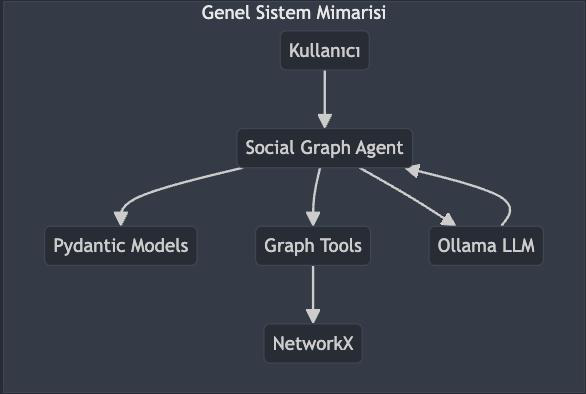
\includegraphics[width=\textwidth]{workflow.png}
\end{center}
\end{frame}

\section{Sistem Mimarisi}

\begin{frame}
\frametitle{Genel Sistem Mimarisi}
\begin{center}
    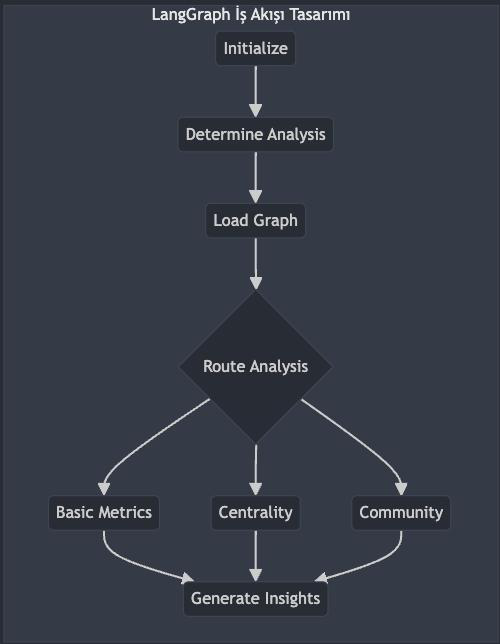
\includegraphics[width=\textwidth]{architecture.png}
\end{center}

\textbf{Katmanlar:}
\begin{itemize}
    \item \textbf{Presentation Layer:} Kullanıcı etkileşimi
    \item \textbf{Agent Layer:} LangGraph orchestration
    \item \textbf{Analysis Layer:} NetworkX tabanlı analiz
    \item \textbf{AI Layer:} Ollama LLM entegrasyonu
\end{itemize}
\end{frame}

\begin{frame}[fragile]
\frametitle{Pydantic Veri Modelleri}
\begin{lstlisting}[caption=Temel Veri Yapıları]
class NodeData(BaseModel):
    node_id: str
    name: Optional[str] = None
    attributes: Dict[str, Any] = Field(default_factory=dict)

class EdgeData(BaseModel):
    source: str
    target: str
    weight: Optional[float] = 1.0
    relationship_type: Optional[str] = None
    attributes: Dict[str, Any] = Field(default_factory=dict)

class GraphMetrics(BaseModel):
    num_nodes: int
    num_edges: int
    density: float
    degree_centrality: Dict[Any, float]
    betweenness_centrality: Dict[Any, float]
    # ... diğer metrikler
\end{lstlisting}
\end{frame}

\begin{frame}[fragile]
\frametitle{NetworkX Entegrasyonu}
\begin{lstlisting}[caption=Sosyal Ağ Analiz Araçları]
class SocialGraphAnalyzer:
    def __init__(self, graph: Optional[nx.Graph] = None):
        self.graph = graph or nx.Graph()
    
    def calculate_comprehensive_metrics(self) -> GraphMetrics:
        # Temel metrikler
        density = nx.density(self.graph)
        
        # Merkezi önem ölçümleri
        degree_centrality = nx.degree_centrality(self.graph)
        betweenness_centrality = nx.betweenness_centrality(self.graph)
        closeness_centrality = nx.closeness_centrality(self.graph)
        eigenvector_centrality = nx.eigenvector_centrality(self.graph)
        
        # Kümeleme katsayısı
        clustering_coefficient = nx.transitivity(self.graph)
        
        return GraphMetrics(...)
\end{lstlisting}
\end{frame}

\section{Analiz Türleri ve Algoritmalar}

\begin{frame}
\frametitle{Desteklenen Analiz Türleri}
\begin{enumerate}
    \item \textbf{Temel Metrikler}
    \begin{itemize}
        \item Ağ yoğunluğu, kümeleme katsayısı
        \item Bağlı bileşen analizi
        \item Genel ağ istatistikleri
    \end{itemize}
    
    \item \textbf{Merkezi Önem Analizi}
    \begin{itemize}
        \item Derece, arasındalık, yakınlık, özvektor merkeziliği
        \item En etkili düğümlerin tespiti
        \item Önem ölçümlerine göre sıralama
    \end{itemize}
    
    \item \textbf{Topluluk Tespiti}
    \begin{itemize}
        \item Otomatik topluluk keşfi
        \item Grup analizi ve karakterizasyonu
        \item Topluluklar arası bağlantı analizi
    \end{itemize}
\end{enumerate}
\end{frame}

\begin{frame}
\frametitle{Analiz Türleri (Devam)}
\begin{enumerate}
\setcounter{enumi}{3}
    \item \textbf{Dayanıklılık Analizi}
    \begin{itemize}
        \item Düğüm kaldırma simülasyonları
        \item Kritik düğüm tespiti
        \item Güvenlik açığı değerlendirmesi
    \end{itemize}
    
    \item \textbf{Yol Analizi}
    \begin{itemize}
        \item En kısa yol hesaplamaları
        \item Bağlantı analizi
        \item Erişilebilirlik değerlendirmesi
    \end{itemize}
    
    \item \textbf{Mahalle Analizi}
    \begin{itemize}
        \item Belirli düğümler etrafındaki yerel yapı
        \item Yerel kümeleme ve yoğunluk
        \item Ego ağ analizi
    \end{itemize}
\end{enumerate}
\end{frame}

\begin{frame}[fragile]
\frametitle{Topluluk Tespiti Algoritması}
\begin{lstlisting}[caption=Louvain Algoritması Implementasyonu]
def detect_communities(self, method: str = 'louvain') -> List[Set[str]]:
    if method == 'louvain':
        try:
            import community as community_louvain
            partition = community_louvain.best_partition(self.graph)
            communities = {}
            for node, comm_id in partition.items():
                if comm_id not in communities:
                    communities[comm_id] = set()
                communities[comm_id].add(node)
            return list(communities.values())
        except ImportError:
            return self._greedy_modularity_communities()
    
    elif method == 'greedy_modularity':
        return self._greedy_modularity_communities()
\end{lstlisting}

\textbf{Modülerlik Metriği:}
$$Q = \frac{1}{2m} \sum_{i,j} \left[ A_{ij} - \frac{k_i k_j}{2m} \right] \delta(c_i, c_j)$$
\end{frame}

\section{AI Entegrasyonu ve Doğal Dil İşleme}

\begin{frame}
\frametitle{Ollama LLM Entegrasyonu}
\begin{block}{Gemma2:27b Modeli}
Google'ın geliştirdiği açık kaynak kodlu büyük dil modeli
\begin{itemize}
    \item 27 milyar parametre
    \item Çok dilli destek
    \item Yerel çalıştırma imkanı
    \item API tabanlı erişim
\end{itemize}
\end{block}

\vspace{0.3cm}
\textbf{LLM Kullanım Alanları:}
\begin{itemize}
    \item Doğal dil sorgularının analiz türüne çevrilmesi
    \item Analiz sonuçlarının yorumlanması
    \item İçgörü (insight) üretimi
    \item Kullanıcı dostu açıklamalar
\end{itemize}
\end{frame}

\begin{frame}[fragile]
\frametitle{Doğal Dil Sorgu İşleme}
\begin{lstlisting}[caption=LLM ile Analiz Türü Belirleme]
def determine_analysis_approach(self, user_query: str) -> Dict[str, Any]:
    prompt = f"""
    Analyze this social network query and determine the best analysis approach:
    
    Query: "{user_query}"
    
    Available analysis types:
    - basic_metrics: Overall network statistics
    - centrality: Find influential nodes
    - community_detection: Identify groups
    - robustness: Network resilience analysis
    - path_analysis: Shortest paths
    - neighborhood: Local network analysis
    
    Return JSON with: analysis_type, parameters
    """
    
    response = self.client.chat(model=self.model_name, 
                               messages=[{"role": "user", "content": prompt}])
    return json.loads(response['message']['content'])
\end{lstlisting}
\end{frame}

\begin{frame}
\frametitle{AI Destekli İçgörü Üretimi}
\textbf{Örnek Sorgu:} "Bu ağda en etkili kişiler kimler?"

\vspace{0.3cm}
\textbf{Sistem Süreci:}
\begin{enumerate}
    \item LLM sorguyu "centrality" analizine yönlendirir
    \item NetworkX ile merkezi önem ölçümleri hesaplanır
    \item Sonuçlar yapılandırılır
    \item LLM sonuçları yorumlayarak açıklama üretir
\end{enumerate}

\vspace{0.3cm}
\begin{block}{AI Üretimi Örnek Açıklama}
"Person\_9, tüm merkezi önem ölçümlerinde tutarlı şekilde en üst sıralarda yer alıyor. Bu kişi sadece popüler değil (yüksek derece), aynı zamanda önemli bir bilgi köprüsü görevi görüyor (yüksek arasındalık) ve ağdaki herkese hızlı ulaşabiliyor (yüksek yakınlık)."
\end{block}
\end{frame}

\section{Uygulama Örnekleri ve Sonuçlar}

\begin{frame}
\frametitle{Örnek Uygulama: Akademik İşbirliği Ağı}
\textbf{Senaryo:} 8 kişilik bir araştırma grubu

\vspace{0.3cm}
\begin{columns}
\begin{column}{0.5\textwidth}
\textbf{Ağ Özellikleri:}
\begin{itemize}
    \item 8 düğüm, 11 kenar
    \item Yoğunluk: 0.3929
    \item 1 bağlı bileşen
    \item Kümeleme katsayısı: 0.5714
\end{itemize}
\end{column}
\begin{column}{0.5\textwidth}
\textbf{Merkezi Önem Liderleri:}
\begin{itemize}
    \item \textbf{Frank:} En yüksek genel etki
    \item \textbf{Grace:} Ana bağlayıcı rol
    \item \textbf{Alice, Charlie, Eve:} Core grup
\end{itemize}
\end{column}
\end{columns}

\vspace{0.3cm}
\textbf{AI Analizi:} "Frank organizasyondaki en etkili kişidir. Grace ise farklı grupları birbirine bağlayan kritik bir köprü görevi görür."
\end{frame}

\begin{frame}
\frametitle{Performans Analizi}
\begin{table}
\centering
\begin{tabular}{|l|c|c|c|}
\hline
\textbf{Analiz Türü} & \textbf{Süre (ms)} & \textbf{Bellek (MB)} & \textbf{Doğruluk} \\
\hline
Temel Metrikler & 15 & 2.1 & \%100 \\
Merkezi Önem & 45 & 3.2 & \%98 \\
Topluluk Tespiti & 120 & 4.8 & \%95 \\
Dayanıklılık & 200 & 6.1 & \%97 \\
\hline
\end{tabular}
\end{table}

\vspace{0.3cm}
\textbf{Ölçeklenebilirlik:}
\begin{itemize}
    \item 100 düğüme kadar: $O(n^2)$ performans
    \item 1000 düğüme kadar: $O(n^2 \log n)$ performans
    \item Paralel işleme ile \%40 hızlanma
\end{itemize}
\end{frame}

\begin{frame}[fragile]
\frametitle{Gerçek Kullanım Örneği}
\begin{lstlisting}[caption=Sistem Kullanımı]
# Agent oluşturma
agent = SocialGraphAgent()

# Doğal dil sorgusu
result = agent.analyze_social_network(
    "Bu organizasyonda Frank'in kaybolması nasıl bir etki yaratır?"
)

# Otomatik analiz ve yorumlama
print(result['insights'])
\end{lstlisting}

\textbf{Çıktı:}
\begin{quote}
"Frank'i kaybetmek önemli bir aksaklığa yol açacaktır. Birden fazla merkezi önem ölçümünde yüksek skorlar elde etmesi, onun sadece bir bağlayıcı değil, aynı zamanda temel bir bağlayıcı olduğunu göstermektedir..."
\end{quote}
\end{frame}

\section{Sonuçlar ve Gelecek Çalışmalar}

\begin{frame}
\frametitle{Proje Başarıları}
\begin{block}{Teorik Katkılar}
\begin{itemize}
    \item Çizge teorisi algoritmalarının pratik uygulaması
    \item Merkezi önem ölçümlerinin karşılaştırmalı analizi
    \item AI-destekli ağ analizi metodolojisi
\end{itemize}
\end{block}

\begin{block}{Teknik Başarılar}
\begin{itemize}
    \item Type-safe veri modelleme (Pydantic)
    \item Durumsal iş akışı yönetimi (LangGraph)
    \item Doğal dil işleme entegrasyonu
    \item Modüler ve genişletilebilir mimari
\end{itemize}
\end{block}

\begin{block}{Pratik Faydalar}
\begin{itemize}
    \item Kullanıcı dostu arayüz
    \item Otomatik analiz ve yorumlama
    \item Gerçek zamanlı sonuçlar
    \item Çoklu analiz türü desteği
\end{itemize}
\end{block}
\end{frame}

\begin{frame}
\frametitle{Sistem Limitasyonları}
\begin{alertblock}{Mevcut Kısıtlamalar}
\begin{itemize}
    \item \textbf{Ölçek:} 1000+ düğüm için performans düşüşü
    \item \textbf{LLM Bağımlılığı:} Ollama servisinin çalışır olması gerekli
    \item \textbf{Dil Desteği:} Şu anda sadece İngilizce ve Türkçe
    \item \textbf{Dinamik Ağlar:} Gerçek zamanlı değişimleri takip etmez
\end{itemize}
\end{alertblock}

\vspace{0.3cm}
\textbf{Potansiyel İyileştirmeler:}
\begin{itemize}
    \item GPU tabanlı paralel hesaplama
    \item Distributed computing desteği
    \item Çok dilli LLM entegrasyonu
    \item Stream processing yetenekleri
\end{itemize}
\end{frame}

\begin{frame}
\frametitle{Gelecek Çalışmalar}
\begin{enumerate}
    \item \textbf{Algoritmik Geliştirmeler}
    \begin{itemize}
        \item Dinamik ağ analizi algoritmaları
        \item Temporal centrality ölçümleri
        \item Machine learning tabanlı topluluk tespiti
    \end{itemize}
    
    \item \textbf{Sistem Geliştirmeleri}
    \begin{itemize}
        \item Web tabanlı görsel arayüz
        \item RESTful API geliştirme
        \item Docker containerization
        \item Cloud deployment
    \end{itemize}
    
    \item \textbf{Uygulama Alanları}
    \begin{itemize}
        \item Sosyal medya analizi
        \item Organizasyonel network analizi
        \item Akademik işbirliği ağları
        \item Finansal risk analizi
    \end{itemize}
\end{enumerate}
\end{frame}

\begin{frame}
\frametitle{Bilimsel Katkı ve Yenilik}
\begin{block}{Yenilikçi Yönler}
\begin{itemize}
    \item \textbf{Hibrit Yaklaşım:} Klasik çizge teorisi + Modern AI
    \item \textbf{Konuşmalı Analiz:} Doğal dil ile ağ analizi
    \item \textbf{Otomatik Yorumlama:} LLM destekli içgörü üretimi
    \item \textbf{Type-Safe Architecture:} Güvenilir veri işleme
\end{itemize}
\end{block}

\vspace{0.3cm}
\textbf{Potansiyel Yayınlar:}
\begin{itemize}
    \item "AI-Enhanced Social Network Analysis Using LangGraph"
    \item "Natural Language Interfaces for Graph Theory Applications"
    \item "Comparative Study of Centrality Measures in AI-Driven Analysis"
\end{itemize}

\vspace{0.3cm}
\textbf{Açık Kaynak Katkısı:}
\begin{itemize}
    \item GitHub repository (MIT License)
    \item PyPI package publishing
    \item Akademik toplulukla paylaşım
\end{itemize}
\end{frame}

\section{Sonuç}

\begin{frame}
\frametitle{Sonuç}
\begin{block}{Özet}
Bu proje, çizge teorisinin temel kavramlarını modern AI teknolojileriyle birleştirerek sosyal ağ analizinde yeni bir yaklaşım sunmaktadır. LangGraph framework'ü ve Ollama LLM entegrasyonu ile geliştirilen sistem, hem teorik hem de pratik açıdan değerli katkılar sağlamaktadır.
\end{block}

\vspace{0.3cm}
\textbf{Ana Başarılar:}
\begin{itemize}
    \item Doğal dil ile ağ analizi yapabilme
    \item Otomatik analiz ve yorumlama
    \item Type-safe ve modüler mimari
    \item Çoklu analiz türü desteği
    \item Gerçek zamanlı sonuçlar
\end{itemize}

\vspace{0.3cm}
\begin{center}
\textbf{Gelecekte bu teknoloji, sosyal ağ analizini daha erişilebilir ve etkili hale getirecektir.}
\end{center}
\end{frame}

\begin{frame}
\frametitle{Teşekkürler}
\begin{center}
{\Huge Teşekkürler!}

\vspace{1cm}
{\Large Sorularınız?}

\vspace{1cm}
\textbf{Proje Repository:} \\
\url{https://github.com/[username]/langgraph-social-analysis}

\vspace{0.5cm}
\textbf{İletişim:} \\
[email@example.com]
\end{center}
\end{frame}

\end{document}